
%Don't forget to delete
%showkeys
%overfullrule
%\date \ber \er \cmt

%------------------------
\documentclass[11pt, letterpaper, dvipdfmx, draft]{book}


%usepackage
%------------------------
\usepackage{amsmath}
\usepackage{amsthm}
%\usepackage[psamsfonts]{amssymb}
\usepackage{color}
\usepackage{ascmac}
\usepackage{amsfonts}
\usepackage{mathrsfs}
\usepackage{mathtools}
\usepackage{amssymb}
\usepackage{graphicx}
\usepackage{fancybox}
%\usepackage{enumerate}
\usepackage{enumitem}
\usepackage{verbatim}
\usepackage{subfigure}
\usepackage{proof}
\usepackage{listings}
\usepackage{otf}
\usepackage{algorithm}
\usepackage{algorithmic}
\usepackage{tikz}
\usetikzlibrary{cd}
\usepackage[all]{xy}
\usepackage{amscd}

\usepackage{pb-diagram}

\usepackage[dvipdfmx]{hyperref}
\usepackage{xcolor}
\definecolor{darkgreen}{rgb}{0,0.45,0} 
\definecolor{darkred}{rgb}{0.75,0,0}
\definecolor{darkblue}{rgb}{0,0,0.6} 
\hypersetup{
    colorlinks=true,
    citecolor=darkgreen,
    linkcolor=darkred,
    urlcolor=darkblue,
}
\usepackage{pxjahyper}

\usepackage{enumitem}

\usepackage{bbm}

% ================================
% パッケージを追加する場合のスペース 
\usepackage{latexsym}
\usepackage{wrapfig}
\usepackage{layout}
\usepackage{url}

\usepackage{okumacro}
%\usepackage{endnotes}
%\usepackage[french]{babel}

%=================================


% --------------------------
% theoremstyle
% --------------------------
\theoremstyle{definition}


% --------------------------
% newtheoem
% --------------------------

% 日本語で定理, 命題, 証明などを番号付きで用いるためのコマンドです. 
% If you want to use theorem environment in Japanece, 
% you can use these code. 
% Attention!
% All theorem enivironment numbers depend on 
% only section numbers.
\newtheorem{Axiom}{公理}[section]
\newtheorem{Definition}[Axiom]{定義}
\newtheorem{Theorem}[Axiom]{定理}
\newtheorem{Proposition}[Axiom]{命題}
\newtheorem{Lemma}[Axiom]{補題}
\newtheorem{Corollary}[Axiom]{系}
\newtheorem{Example}[Axiom]{例}
\newtheorem{Claim}[Axiom]{主張}
\newtheorem{Property}[Axiom]{性質}
\newtheorem{Attention}[Axiom]{注意}
\newtheorem{Question}[Axiom]{問}
\newtheorem{Problem}[Axiom]{問題}
\newtheorem{Consideration}[Axiom]{考察}
\newtheorem{Alert}[Axiom]{警告}
\newtheorem{Fact}[Axiom]{事実}


% 日本語で定理, 命題, 証明などを番号なしで用いるためのコマンドです. 
% If you want to use theorem environment with no number in Japanese, You can use these code.
\newtheorem*{Axiom*}{公理}
\newtheorem*{Definition*}{定義}
\newtheorem*{Theorem*}{定理}
\newtheorem*{Proposition*}{命題}
\newtheorem*{Lemma*}{補題}
\newtheorem*{Example*}{例}
\newtheorem*{Corollary*}{系}
\newtheorem*{Claim*}{主張}
\newtheorem*{Property*}{性質}
\newtheorem*{Attention*}{注意}
\newtheorem*{Question*}{問}
\newtheorem*{Problem*}{問題}
\newtheorem*{Consideration*}{考察}
\newtheorem*{Alert*}{警告}
\newtheorem{Fact*}{事実}


% 英語で定理, 命題, 証明などを番号付きで用いるためのコマンドです. 
% If you want to use theorem environment in English, You can use these code.
%all theorem enivironment number depend on only section number.
\newtheorem{Axiom+}{Axiom}[section]
\newtheorem{Definition+}[Axiom+]{Definition}
\newtheorem{Theorem+}[Axiom+]{Theorem}
\newtheorem{Proposition+}[Axiom+]{Proposition}
\newtheorem{Lemma+}[Axiom+]{Lemma}
\newtheorem{Example+}[Axiom+]{Example}
\newtheorem{Corollary+}[Axiom+]{Corollary}
\newtheorem{Claim+}[Axiom+]{Claim}
\newtheorem{Property+}[Axiom+]{Property}
\newtheorem{Attention+}[Axiom+]{Attention}
\newtheorem{Question+}[Axiom+]{Question}
\newtheorem{Problem+}[Axiom+]{Problem}
\newtheorem{Consideration+}[Axiom+]{Consideration}
\newtheorem{Alert+}{Alert}
\newtheorem{Fact+}[Axiom+]{Fact}
\newtheorem{Remark+}[Axiom+]{Remark}

% ----------------------------
% commmand
% ----------------------------
% 執筆に便利なコマンド集です. 
% コマンドを追加する場合は下のスペースへ. 

% 集合の記号 (黒板文字)
\newcommand{\NN}{\mathbb{N}}
\newcommand{\ZZ}{\mathbb{Z}}
\newcommand{\QQ}{\mathbb{Q}}
\newcommand{\RR}{\mathbb{R}}
\newcommand{\CC}{\mathbb{C}}
\newcommand{\PP}{\mathbb{P}}
\newcommand{\KK}{\mathbb{K}}


% 集合の記号 (太文字)
\newcommand{\nn}{\mathbf{N}}
\newcommand{\zz}{\mathbf{Z}}
\newcommand{\qq}{\mathbf{Q}}
\newcommand{\rr}{\mathbf{R}}
\newcommand{\cc}{\mathbf{C}}
\newcommand{\pp}{\mathbf{P}}
\newcommand{\kk}{\mathbf{K}}

% 特殊な写像の記号
\newcommand{\ev}{\mathop{\mathrm{ev}}\nolimits} % 値写像
\newcommand{\pr}{\mathop{\mathrm{pr}}\nolimits} % 射影

% スクリプト体にするコマンド
%   例えば {\mcal C} のように用いる
\newcommand{\mcal}{\mathcal}

% 花文字にするコマンド 
%   例えば {\h C} のように用いる
\newcommand{\h}{\mathscr}

%筆記体
\newcommand{\cA}{\mcal{A}}
\newcommand{\cB}{\mcal{B}}
\newcommand{\cC}{\mcal{C}}
\newcommand{\cD}{\mcal{D}}
\newcommand{\cE}{\mcal{E}}
\newcommand{\cF}{\mcal{F}}
\newcommand{\cG}{\mcal{G}}
\newcommand{\cH}{\mcal{H}}
\newcommand{\cI}{\mcal{I}}
\newcommand{\cJ}{\mcal{J}}
\newcommand{\cK}{\mcal{K}}
\newcommand{\cL}{\mcal{L}}
\newcommand{\cM}{\mcal{M}}
\newcommand{\cN}{\mcal{N}}
\newcommand{\cO}{\mcal{O}}
\newcommand{\cP}{\mcal{P}}
\newcommand{\cQ}{\mcal{Q}}
\newcommand{\cR}{\mcal{R}}
\newcommand{\cS}{\mcal{S}}
\newcommand{\cT}{\mcal{T}}
\newcommand{\cU}{\mcal{U}}
\newcommand{\cV}{\mcal{V}}
\newcommand{\cW}{\mcal{W}}
\newcommand{\cX}{\mcal{X}}
\newcommand{\cY}{\mcal{Y}}
\newcommand{\cZ}{\mcal{Z}}

\newcommand{\rmD}{\mathrm{D}}


\newcommand{\scA}{\mathscr{A}}
\newcommand{\scB}{\mathscr{B}}
\newcommand{\scC}{\mathscr{C}}
\newcommand{\scD}{\mathscr{D}}
\newcommand{\scE}{\mathscr{E}}
\newcommand{\scF}{\mathscr{F}}
\newcommand{\scN}{\mathscr{N}}
\newcommand{\scO}{\mathscr{O}}
\newcommand{\scR}{\mathscr{R}}
\newcommand{\scP}{\mathscr{P}}
\newcommand{\scS}{\mathscr{S}}
\newcommand{\scV}{\mathscr{V}}

\newcommand{\ibA}{\mathop{\text{\textit{\textbf{A}}}}}
\newcommand{\ibB}{\mathop{\text{\textit{\textbf{B}}}}}
\newcommand{\ibC}{\mathop{\text{\textit{\textbf{C}}}}}
\newcommand{\ibD}{\mathop{\text{\textit{\textbf{D}}}}}
\newcommand{\ibE}{\mathop{\text{\textit{\textbf{E}}}}}
\newcommand{\ibF}{\mathop{\text{\textit{\textbf{F}}}}}
\newcommand{\ibG}{\mathop{\text{\textit{\textbf{G}}}}}
\newcommand{\ibH}{\mathop{\text{\textit{\textbf{H}}}}}
\newcommand{\ibI}{\mathop{\text{\textit{\textbf{I}}}}}
\newcommand{\ibJ}{\mathop{\text{\textit{\textbf{J}}}}}
\newcommand{\ibK}{\mathop{\text{\textit{\textbf{K}}}}}
\newcommand{\ibL}{\mathop{\text{\textit{\textbf{L}}}}}
\newcommand{\ibM}{\mathop{\text{\textit{\textbf{M}}}}}
\newcommand{\ibN}{\mathop{\text{\textit{\textbf{N}}}}}
\newcommand{\ibO}{\mathop{\text{\textit{\textbf{O}}}}}
\newcommand{\ibP}{\mathop{\text{\textit{\textbf{P}}}}}
\newcommand{\ibQ}{\mathop{\text{\textit{\textbf{Q}}}}}
\newcommand{\ibR}{\mathop{\text{\textit{\textbf{R}}}}}
\newcommand{\ibS}{\mathop{\text{\textit{\textbf{S}}}}}
\newcommand{\ibT}{\mathop{\text{\textit{\textbf{T}}}}}
\newcommand{\ibU}{\mathop{\text{\textit{\textbf{U}}}}}
\newcommand{\ibV}{\mathop{\text{\textit{\textbf{V}}}}}
\newcommand{\ibW}{\mathop{\text{\textit{\textbf{W}}}}}
\newcommand{\ibX}{\mathop{\text{\textit{\textbf{X}}}}}
\newcommand{\ibY}{\mathop{\text{\textit{\textbf{Y}}}}}
\newcommand{\ibZ}{\mathop{\text{\textit{\textbf{Z}}}}}

\newcommand{\ibx}{\mathop{\text{\textit{\textbf{x}}}}}

\newcommand{\Comp}{\mathop{\mathrm{C}}\nolimits}
\newcommand{\Komp}{\mathop{\mathsf{K}}\nolimits}
\newcommand{\Domp}{\mathsf{D}}
\newcommand{\Kompl}{\mathop{\mathsf{K}^\mathrm{+}}\nolimits}
\newcommand{\Kompu}{\mathop{\mathsf{K}^\mathrm{-}}\nolimits}
\newcommand{\Kompb}{\mathop{\mathsf{K}^\mathrm{b}}\nolimits}
\newcommand{\Dompl}{\mathop{\mathsf{D}^\mathrm{+}}\nolimits}
\newcommand{\Dompu}{\mathop{\mathsf{D}^\mathrm{-}}\nolimits}
\newcommand{\Dompb}{\mathop{\mathsf{D}^\mathrm{b}}\nolimits}

\newcommand{\CCat}{\Comp(\cat)}
\newcommand{\KCat}{\Komp(\cat)}
\newcommand{\DCat}{\Domp(\cat)}%圏Cの複体のホモトピー圏
\newcommand{\HOM}{\mathop{\mathscr{H}\hspace{-2pt}om}\nolimits}%内部Hom
\newcommand{\RHOM}{\mathop{\mathrm{R}\hspace{-1.5pt}\HOM}\nolimits}

\newcommand{\muS}{\mathop{\mathrm{SS}}\nolimits}
\newcommand{\RG}{\mathop{\mathrm{R}\hspace{-0pt}\Gamma}\nolimits}
\newcommand{\RHom}{\mathop{\mathrm{R}\hspace{-1.5pt}\Hom}\nolimits}
\newcommand{\Rder}{\mathrm{R}}

\newcommand{\simar}{\mathrel{\overset{\sim}{\longrightarrow}}}%内部Hom
\newcommand{\simra}{\mathrel{\overset{\sim}{\longleftarrow}}}%内部Hom

% 偏微分作用素の記号
\newcommand{\p}{\partial}

% 角カッコの記号 (内積は下にマクロがあります)
\newcommand{\lan}{\langle}
\newcommand{\ran}{\rangle}



% 圏の記号など
\newcommand{\Set}{{\bf Set}}
\newcommand{\Vect}{{\bf Vect}}
\newcommand{\FDVect}{{\bf FDVect}}
\newcommand{\Ring}{{\bf Ring}}
\newcommand{\Ab}{{\bf Ab}}
\newcommand{\Mod}{\mathop{\mathrm{Mod}}\nolimits}
\newcommand{\CGA}{{\bf CGA}}
\newcommand{\GVect}{{\bf GVect}}
\newcommand{\Lie}{{\bf Lie}}
\newcommand{\dLie}{{\bf Liec}}

\newcommand{\indlim}[1][]{\mathop{\varinjlim}\limits_{#1}}
\newcommand{\sindlim}[1][]{\smash{\mathop{\varinjlim}\limits_{#1}}\,}
\newcommand{\Pro}{\mathrm{Pro}}
\newcommand{\Ind}{\mathrm{Ind}}
\newcommand{\prolim}[1][]{\mathop{\varprojlim}\limits_{#1}}
\newcommand{\sprolim}[1][]{\smash{\mathop{\varprojlim}\limits_{#1}}\,}


% 射の集合など
\newcommand{\Map}{\mathop{\mathrm{Map}}\nolimits}
\newcommand{\Hom}{\mathop{\mathrm{Hom}}\nolimits}
\newcommand{\End}{\mathop{\mathrm{End}}\nolimits}
\newcommand{\Aut}{\mathop{\mathrm{Aut}}\nolimits}
\newcommand{\Mor}{\mathop{\mathrm{Mor}}\nolimits}

% その他便利なコマンド
\newcommand{\dip}{\displaystyle} % 本文中で数式モード
\newcommand{\e}{\varepsilon} % イプシロン
\newcommand{\dl}{\delta} % デルタ
\newcommand{\pphi}{\varphi} % ファイ
\newcommand{\ti}{\tilde} % チルダ
\newcommand{\pal}{\parallel} % 平行
\newcommand{\op}{{\rm op}} % 双対を取る記号
\newcommand{\lcm}{\mathop{\mathrm{lcm}}\nolimits} % 最小公倍数の記号
\newcommand{\Probsp}{(\Omega, \F, \P)} 
\newcommand{\argmax}{\mathop{\rm arg~max}\limits}
\newcommand{\argmin}{\mathop{\rm arg~min}\limits}





% ================================
% コマンドを追加する場合のスペース 
\newcommand{\UU}{\mcal{U}}
\newcommand{\OO}{\mcal{O}}
\newcommand{\emp}{\varnothing}
\newcommand{\ceq}{\coloneqq}
\newcommand{\sbs}{\subset}
\newcommand{\mapres}[2]{\left. #1 \right|_{#2}}
\newcommand{\ded}{\hfill $\blacksquare$}
\newcommand{\id}{\mathrm{id}}
\newcommand{\isom}{\overset{\sim}{\longrightarrow}}
\newcommand{\tTop}{\textsf{Top}}
\newcommand{\pfb}{\textbf{証明}}
\newcommand{\Int}{\mathop{\mathrm{Int}}\nolimits} % 内部


% 自前の定理環境
%   https://mathlandscape.com/latex-amsthm/
% を参考にした
\newtheoremstyle{mystyle}%   % スタイル名
    {5pt}%                   % 上部スペース
    {5pt}%                   % 下部スペース
    {}%              % 本文フォント
    {}%                  % 1行目のインデント量
    {\bfseries}%                      % 見出しフォント
    {.}%                     % 見出し後の句読点
    {12pt}%                     % 見出し後のスペース
    {\thmname{#1}\thmnumber{ #2 }\thmnote{{\normalfont (#3)}}}% % 見出しの書式

\theoremstyle{mystyle}
\newtheorem{AXM}{公理}[section]
\newtheorem{DFN}[Axiom]{定義}
\newtheorem{THM}[Axiom]{定理}
\newtheorem*{THM*}{定理}
\newtheorem{PRP}[Axiom]{命題}
\newtheorem{LMM}[Axiom]{補題}
\newtheorem{CRL}[Axiom]{系}
\newtheorem{EG}[Axiom]{例}

%\newtheorem{}{Axiom}[]
\numberwithin{equation}{section} % 式番号を「(3.5)」のように印刷

\newcommand{\MM}{\mcal{M}}
\newcommand{\bk}{\mathbf{k}}

% =================================


% ---------------------------
% new definition macro
% ---------------------------
% 便利なマクロ集です

% 内積のマクロ
%   例えば \inner<\pphi | \psi> のように用いる
\def\inner<#1>{\langle #1 \rangle}

% ================================
% マクロを追加する場合のスペース 

%=================================





% ----------------------------
% documenet 
% ----------------------------
% 以下, 本文の執筆スペースです. 
% Your main code must be written between 
% begin document and end document.
% ---------------------------




\begin{document}

\title{Systems of Microdifferential Equations}
%\author{Pierre Schapira}
\date{}
\maketitle
\frontmatter
\tableofcontents
\layout

\chapter{Introduction}

This book is grew out from a course that 
Masaki Kashiwara gave at the ``Universit\'e Paris-Nord'' 
during the first term of the academic year 1976--77. 
Teresa Monterio Fernandes worked out lecture notes for 
this course, which were preprinted in 1979 by Paris-Nord 
under the title ``Syst\`ems d'\'equations 
microdiff\'erentielles'' and distributed to a happy few. 
On the grounds that such a basic textbook 
should be made available to a wider mathematical audience, 
the Birkh\"auser Publishing Company proposed to make it 
a new volume of its series ``Progress in Mathematics''. 
Kashiwara and the publisher agreed not to change the overall 
structure of the text (which at first 
was supposed to be provisional); T. Monterio Fernandes then 
was kind enough to make care of the translation into English 
and of the necessary minor corrections. 

It was decided that an introduction might be written, outlining 
the purposes and main features of the text, and mentioning 
recent developments connected with the index fomula in Chapter \ref{ch6}. 
Kashiwara suggested that I would write this introduction, 
and I accepted to do so with pleasure. 
I thought it might be a way of thanking Kashiwara for 
all he has taught me since I benefited so much from 
talking to him and reading his works. 

In short, this book is an introduction to systems of 
microdifferential equations and to some of the tools 
of micro-local analysis. 
Here a remark on the terminology; after \cite{BK76}, 
pseudo-differential operators on a complex manifold \(X\) 
were considered in \cite{SKK}: 
They used the notation \(\cP_X\) for the sheaf of rings 
of pseudo-differential operators (this was a sheaf on the 
projectivised cotangent bundles of \(X\)). 
In recent years, instead \(\cP_X\), 
one has been using \(\cE_X\) (now viewed as a sheaf of rings 
on the cotangent bundle itself); \(\cE_X\) is called 
the sheaf of \emph{micro-differential operators}: 
micro-differential operators are defined and studied 
locally in the cotangent bundle, i.e. \emph{microlocally}. 

As is well-known, say for \(X\) of complex dimension one 
with variable \(t\), 
both \(\frac{d}{dt}\) and \(
    \left(\frac{d}{dt}\right)^{-1}
\) are micro-differential operators (more precisely, 
as a section of \(\cE_X\), 
\(\left(\frac{d}{dt}\right)^{-1}\) is defined outside the
zero-section of the cotangent bundle). 
An infinite series \(
    \sum_{n\geqq0}^{}a_n(t)\left(\frac{d}{dt}\right)^{-n}
\) also defines a micro-differential operator, providing 
the holomorphic functions \(a_n(t)\) satisfy, 
on any compact \(K\) of \(X\), an estimate of the type 
\[
    \sup_{t\in K}\lvert a_n(t)\rvert < (n!)C_K^n,\quad\text{for~some \(C_K>0\).}
\]
There is no way to make such operators act on the space of 
holomorphic functions. However, 
let \(X=\cc\) and 
take a closed angular sector \(Z_\varepsilon\) inside 
the disk \(
    D_\varepsilon=\{t\in \cc; \lvert t\rvert <\varepsilon\}
\).
\begin{figure}[htb]
    \centering
    %\scalebox{0.8}{
        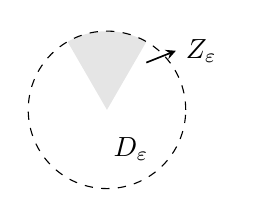
\begin{tikzpicture}[x=0.5cm,y=0.5cm]
        \fill[black!10] (1,1.73)arc(60:120:2)--(-1,1.73)-- (0,0)--cycle;
        \draw[dashed,black!100] (0.7,0.1) (0,0) ellipse (2 and 2);
        \draw[->,>=stealth,semithick] (1,1.2)--(1.75,1.5)node[right]{$Z_\varepsilon$}; %x軸
        \draw (1.3,-1) node[left]{$D_\varepsilon$};
    \end{tikzpicture}%}
    %\caption{開区間は円盤と閉区間の合併}
    %\label{fig:loc-closed-intersection}
\end{figure}\\%
Let \(\cO(D_\varepsilon)\) resp.~\(
    \cO(D_\varepsilon-Z_\varepsilon)
\) be the space of holomorphic functions on \(D_\varepsilon\) 
resp.~\(D_\varepsilon-Z_\varepsilon\); 
then \(\left(\frac{d}{dt}\right)^{-1}\) operates on \(
    \cO(D_\varepsilon-Z_\varepsilon)\mathbin{|}\cO(D_\varepsilon)
\), to get an operation of microdifferential operators,
it suffices to make \(\varepsilon\) smaller and smaller, i.e. 
to consider \(
    \indlim[\varepsilon\to0]
    \cO(D_\varepsilon-Z_\varepsilon)
    \mathbin{|}
    \cO(D_\varepsilon)
\).

The reader will find two definitions 


\mainmatter
\chapter{Microfunctions}\label{ch1}
\chapter{Microdifferential Systems}\label{ch2}
\chapter{Structure of Coherent $\mcal{E}_X$-modules}\label{ch3}
\chapter{Holomorphic Solutions of Systems of Partial Differential Equations}\label{ch4}
\chapter{Solutions of Holonomic Systems}\label{ch5}
\chapter{Index Theorems}\label{ch6}
\appendix
\chapter{Derived Categories and Functors}\label{chA}
\chapter{Whitney Stratification and Constructible Sheaves}\label{chB}


\backmatter



















\begin{thebibliography}{15}
    \bibitem[Arn67]{Arn67} Vladimir I. Arnold, 
    \textit{On a characteristic class entering into conditions of quantization}, 
    Funkcional. Anal. i Prilozen (1967), 1–14. in Russian.
    \bibitem[Gab81]{Gab81}
    Ofer Gabber, \textit{The integrability of the characteristic variety}, 
    Amer. Journ. Math. 103 (1981), 445-–468.
    \bibitem[GKS12]{GKS12} 
    Stéphane Guillermou, Masaki Kashiwara and Pierre Schapira, 
    \textit{Sheaf quantization of Hamiltonian isotopies and applications to nondisplaceability problems}, 
    Duke Math. J. 161(2): 201--245 (2012).
    \bibitem[KS90]{KS90} Masaki Kashiwara and Pierre Schapira, 
    \textit{Sheaves on manifolds}, Grundlehren der Mathematischen Wissenschaften, 
    vol. 292, Springer-Verlag, Berlin, 1990.
    \bibitem[Ler76]{Ler76} 
    Jean Leray, \textit{Analyse Lagrangienne et m\'ecanique quantique}, 
    Coll\`ege de France, 1976.
    \bibitem[Mas65]{Mas65} Viktor P. Maslov, 
    \textit{Theory of perturbations and asymptotic methods}, 
    Moskow Gos. Univ., 1965.
    [邦訳] マスロフ, 摂動論と漸近的方法, 岩波書店, 1976年.
    \bibitem[Sch21]{Sch21} 
    Pierre Schapira, 
    \textit{Microlocal analysis and beyond}, 
    New spaces in Mathematics, edited by Mathieu Anel 
    and Gabriel Catren, 
    Cambridge University Press, 2021, pp. 117--152.
    \bibitem[44]{SKK}
    Mikio Sato, Takahiro Kawai, and Masaki Kashiwara, 
    \textit{Microfunctions and pseudo-differential equations}, 
    Hyperfunctions and pseudo-differential equations 
    (Proc. Conf., Katata, 1971; dedicated to the memory of 
    Andr\'e Martineau), 
    Springer, Berlin, 1973, pp. 265–-529. 
    Lecture Notes in Math., Vol. 287.

\end{thebibliography}

\begin{thebibliography}{15}
    \bibitem[Boutet de Monvel-Kree]{BK76} 
    Boutet de Monvel, L.; Kree,: 
    \textit{Pseudo-differential operators and Geverey classes}, 
    Ann. Inst. Fourier Grenoble, t.26, 1, p.81--140. (1976)
\end{thebibliography}
%\bibliographystyle{junsrt}
%\bibliography{ref}

\end{document}


